\section{Application with the MOLE library}

\begin{frame}
	\frametitle{\secname}
	\begin{example}[Homogeneous]
		Let's consider the program~\href{https://raw.githubusercontent.com/carlosal1015/mole_examples/main/examples/octave/hyperbolic1D.m}{\mintinline{octave}|hyperbolic1D.m|} subject to the following configuration.
		\begin{equation*}
			\left\{
			\begin{aligned}
				\difcp{u}{t}\left(x,t\right)+
				a\difcp{u}{x}\left(x,t\right) & =
				0,                            & x\in\left(0,1\right), t\in\left(0,1\right). \\
				u\left(0,t\right)             & =
				u\left(1,t\right)=0,          & t\in\left(0,1\right).                       \\
				u\left(x,0\right)             & =
				\sin\left(2\pi x\right),      & x\in\left(0,1\right).
			\end{aligned}
			\right.
		\end{equation*}
		The exact solution is given by
		\begin{equation*}
			u\left(x,t\right)=
			\sin
			\left(2\pi\left(x-at\right)\right).
		\end{equation*}
	\end{example}

	\begin{block}{Leapfrog scheme}
		\begin{equation*}
			u^{n+1}_{i}=
			u^{n}_{i}-
			\frac{c\Delta t}{\Delta x}
			\left(u^{n}_{i+1}-u^{n}_{i-1}\right)+
			\mathcal{O}\left(\Delta t^{2},\Delta x^{2}\right).
		\end{equation*}
	\end{block}

	\begin{alertblock}{CFL condition}
		Using von Neumann stability analysis it can be shown that the
		Leapfrog scheme is stable when
		\begin{equation*}
			\frac{\left|c\right|\Delta t}{\Delta x}\leq 1.
		\end{equation*}
	\end{alertblock}
\end{frame}

\section{Program~\mintinline{octave}|hyperbolic1D.m| with the MOLE library}

\begin{frame}
	\frametitle{\secname}
	\begin{listing}[H]
		\tiny
		\centering
		\pathinputminted[frame=single,framesep=10pt,linenos,firstline=1,lastline=32,highlightlines={18}]{octave}{hyperbolic1D.m}
	\end{listing}
\end{frame}

\begin{frame}
	\frametitle{\secname}
	\begin{listing}[H]
		\tiny
		\centering
		\pathinputminted[frame=single,framesep=10pt,linenos,firstline=34,lastline=68,highlightlines={55}]{octave}{hyperbolic1D.m}
	\end{listing}
\end{frame}

\section{Program~\mintinline{cpp}|hyperbolic1D_upwind.cpp| with the MOLE library}

\begin{frame}
	\frametitle{\secname}
	\begin{listing}[H]
		\tiny
		\centering
		\pathinputminted[frame=single,framesep=10pt,linenos,firstline=1,lastline=35,highlightlines={11-32}]{cpp}{hyperbolic1D_upwind.cpp}
	\end{listing}
\end{frame}

\begin{frame}
	\frametitle{\secname}
	\begin{listing}[H]
		\tiny
		\centering
		\pathinputminted[frame=single,framesep=10pt,linenos,firstline=37,lastline=71,highlightlines={52-53}]{cpp}{hyperbolic1D_upwind.cpp}
	\end{listing}
\end{frame}

\begin{frame}
	\frametitle{\secname}
	\begin{listing}[H]
		\tiny
		\centering
		\pathinputminted[frame=single,framesep=10pt,linenos,firstline=72,lastline=108,highlightlines={107}]{cpp}{hyperbolic1D_upwind.cpp}
	\end{listing}
\end{frame}

\section{Program's overview}

\begin{frame}
	\frametitle{\secname}

	\begin{equation*}
		I\in\mathbb{R}^{\left(m+1\right)\times\left(m+2\right)}.
	\end{equation*}

	\begin{equation*}
		D\in\mathbb{R}^{\left(m+2\right)\times\left(m+1\right)}.
	\end{equation*}
	\href{https://carlosal1015.github.io/mole_examples/api_docs/matlab/src/matlab/interpol.html}{\mintinline{octave}|interpol|}
	\href{https://carlosal1015.github.io/mole_examples/api_docs/matlab/src/matlab/div.html}{\mintinline{octave}|div|}

	\begin{itemize}
		\item

		      The domain $\left[0,1\right]$ is divided with $50$
		      cells, $\Delta x=0.02$.

		\item

		      The CFL condition ensure that stability for explicit
		      schemes.

		\item

		      We use the divergence operator of order $2$.

		\item

		      We use the $1$D interpolation operator of order $2$.

		\item

		      The initial condition is
		      \begin{math}
			      u\left(x,0\right)=
			      \sin\left(2\pi x\right)
		      \end{math}.

		\item

		      We modify the first and last row for the divergence
		      operator in order to impose the periodic boundary conditions.

		\item

		      The spatial operator mixes the divergence and
		      interpolation operators for approximate $-a\difcp{}{x}$.

		\item

		      The factor $2$ fixes the scale in the staggered grid.
	\end{itemize}
\end{frame}

\section{Results}

\begin{frame}
	\frametitle{\secname}
	\begin{figure}[H]
		\centering
		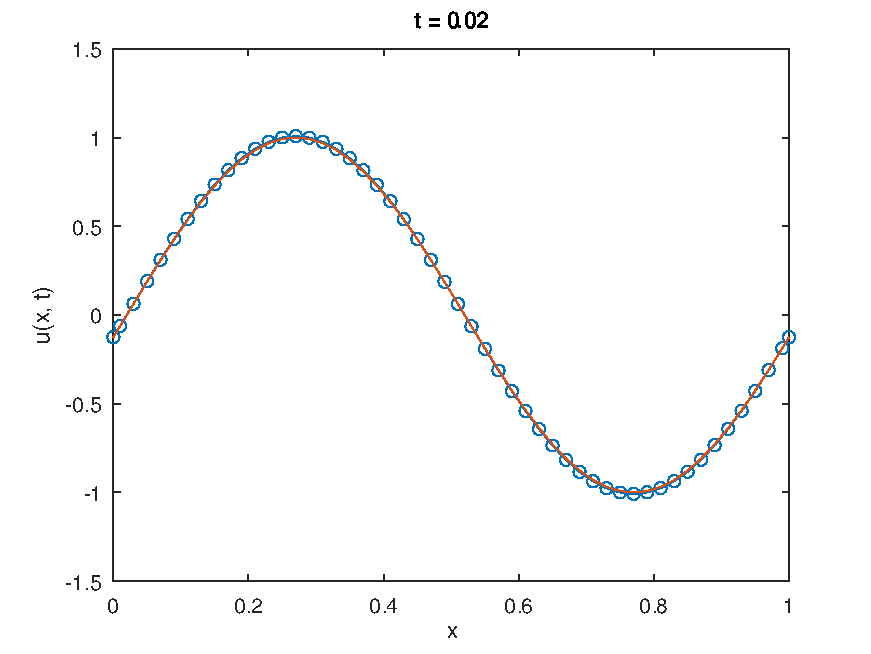
\includegraphics[width=.37\paperwidth]{hyperbolic1D1.pdf}
		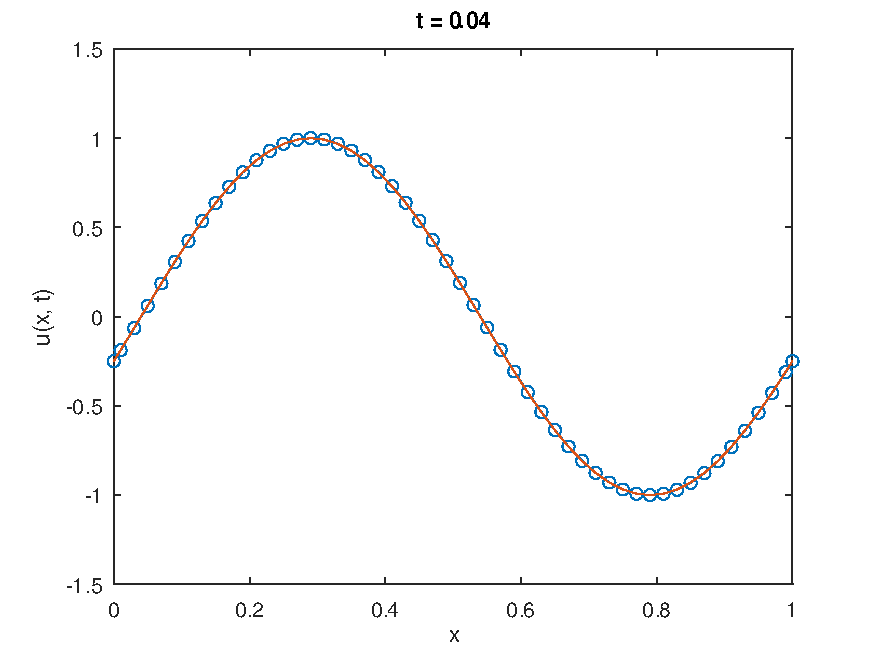
\includegraphics[width=.37\paperwidth]{hyperbolic1D2.pdf}

		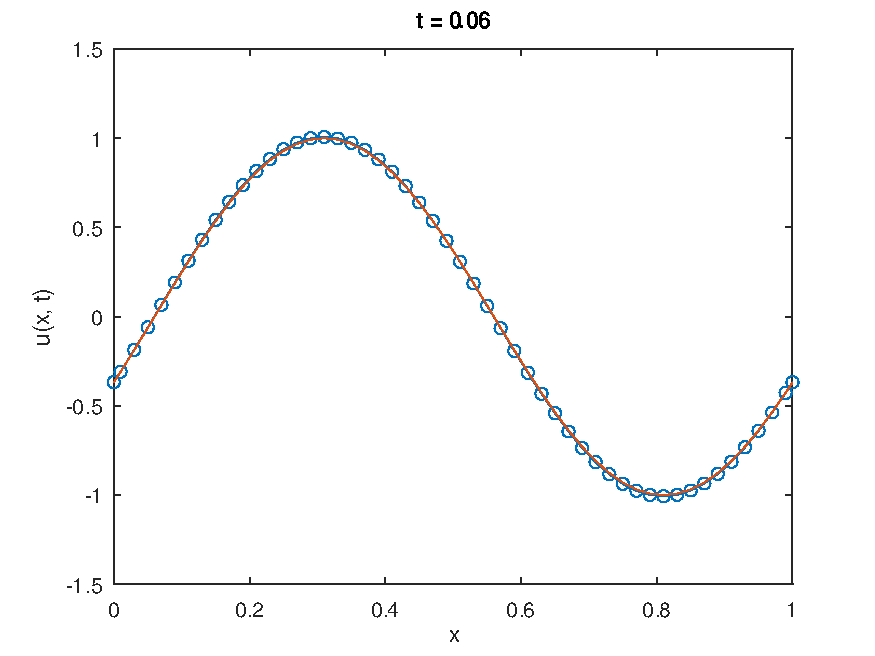
\includegraphics[width=.37\paperwidth]{hyperbolic1D3.pdf}
		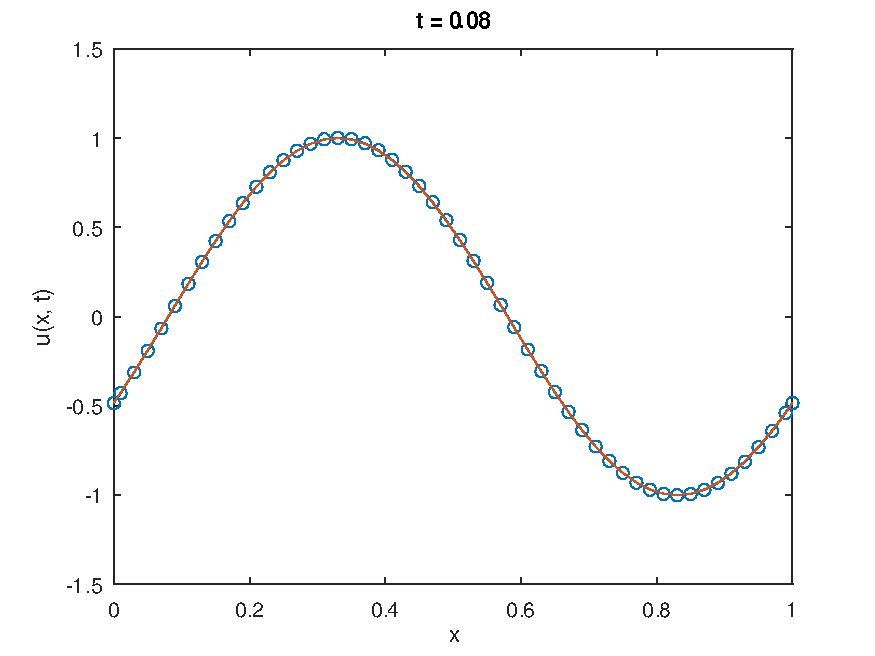
\includegraphics[width=.37\paperwidth]{hyperbolic1D4.pdf}
	\end{figure}
\end{frame}

\begin{frame}
	\frametitle{\secname}
	\begin{figure}[H]
		\centering
		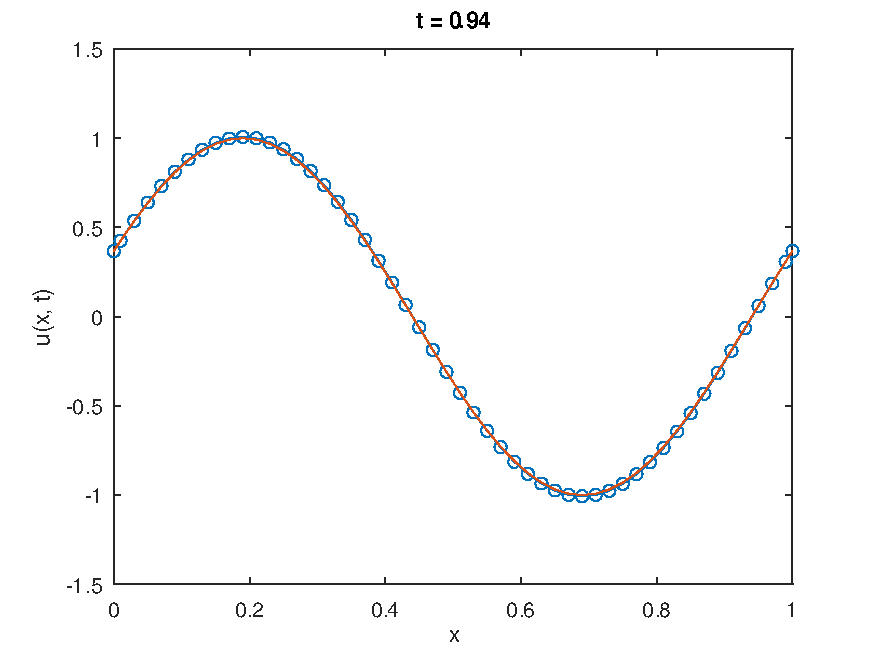
\includegraphics[width=.37\paperwidth]{hyperbolic1D47.pdf}
		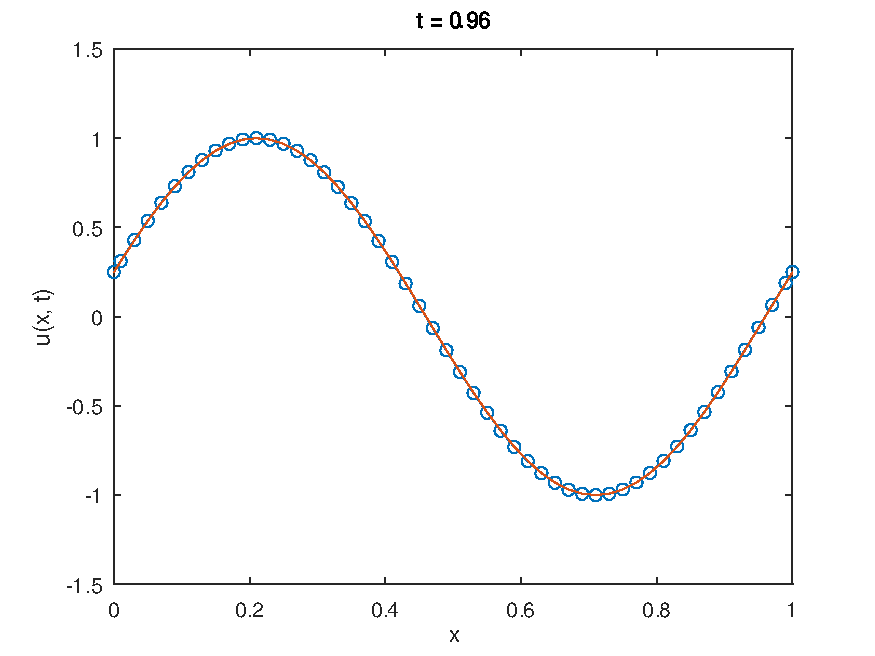
\includegraphics[width=.37\paperwidth]{hyperbolic1D48.pdf}

		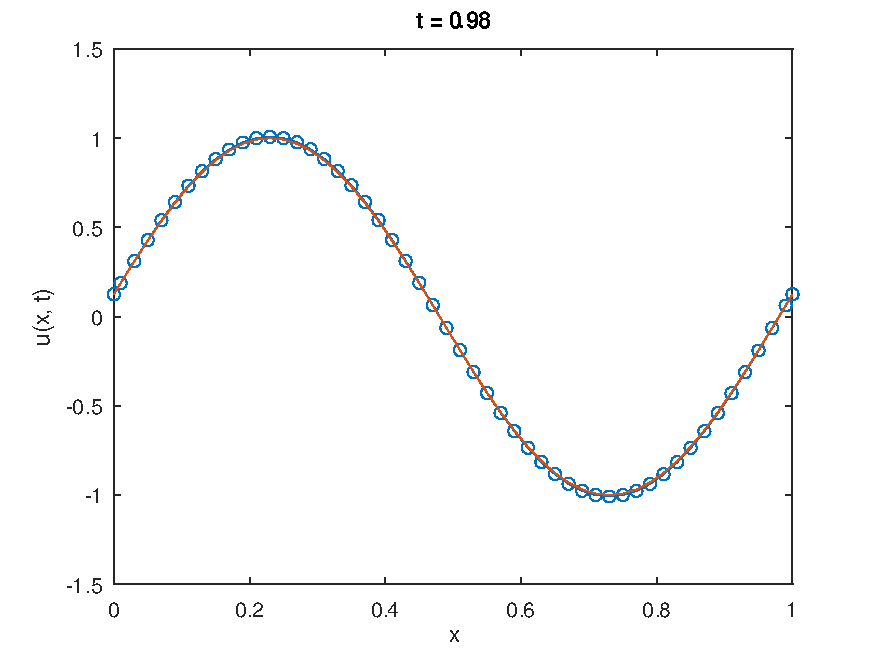
\includegraphics[width=.37\paperwidth]{hyperbolic1D49.pdf}
		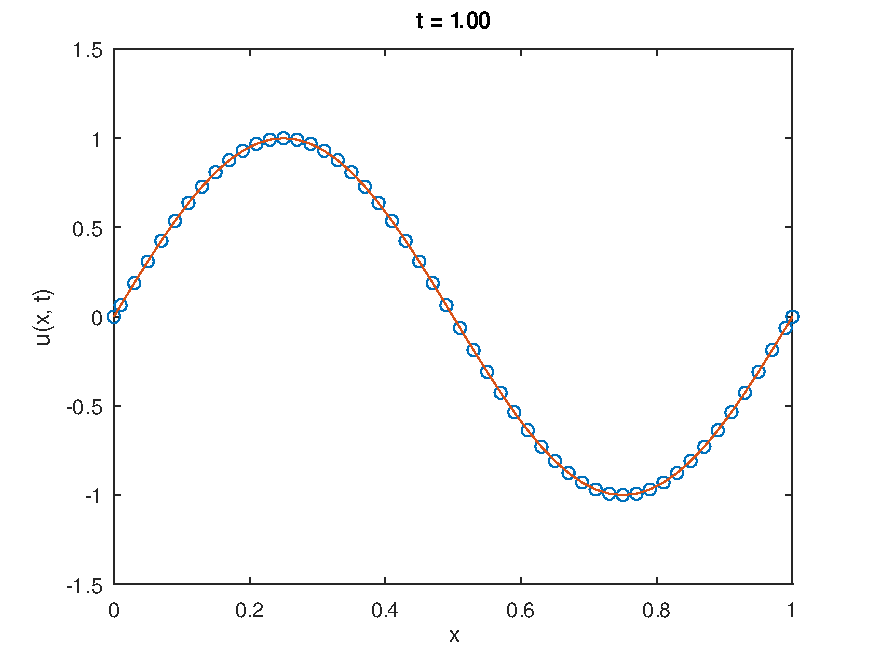
\includegraphics[width=.37\paperwidth]{hyperbolic1D50.pdf}
	\end{figure}
\end{frame}
